\chapter{Експеримент}

\section{Набір даних MNIST}

В цьому розділі ми проведемо експерименти з використанням набору даних MNIST.
Цей набір даних містить 70000 зображень рукописних цифр від 0 до 9, розміром $28
\times 28$ пікселів. Він широко використовується для навчання та тестування
алгоритмів комп'ютерного зору та машинного навчання. В даному експерименті ми
будемо використовувати 60000 зображень для навчання та 10000 зображень для
тестування. Кожне зображення є чорно-білим, і його пікселі мають значення від 0
до 255, де 0 --- це чорний колір, а 255 --- білий. Проте, ці значення пікселів
при нормалізуємо на відрізок $[0,1]$ для стабілізації процесу тренування. Набір
даних MNIST є стандартним набором даних для оцінки алгоритмів класифікації
зображень, тому він ідеально підходить для нашого експерименту. Приклади
зображень з набору даних MNIST були наведені на початку роботи, на
Рисунку~\ref{fig:digits}.

\section{Архітектура нейронної мережі та результати}

В нашому експерименті ми будемо використовувати нейронну мережу, що складається
з трьох конволюційних шарів KAN та одного лінійного шару на виході. 
Архітектура проілюстрована на Рисунку~\ref{fig:kan-arch}.
\begin{figure}
    \centering
    \tikzset{
        base/.style={
            draw,
            rectangle,
            minimum width=5cm,
            minimum height=1cm,
            ultra thick,
            rounded corners=15pt
        },
        maxpool/.style={
            base,
            fill=orange!10,
            draw=orange!90!black
        },
        kanconv/.style={
            base,
            fill=blue!10,
            draw=blue!80!black
        },
        fc/.style={
            base,
            fill=green!10,
            draw=green!70!black
        }
    }
    \begin{tikzpicture}
        % Input
        \node[base] (input) {\textbf{Вхід}};
        \node[left=1cm of input, thick] (image) {
\includegraphics[width=1.75cm]{figures/mnist/digit5.png}};
        \draw[thick, line width=1.5pt, -{Stealth[length=7pt, width=7pt]}] (image) -- (input);
        \node[above=0.1cm of image] {\textcolor{gray}{$\boldsymbol{X} \in \mathbb{R}^{28 \times 28 \times 1}$}};

        \node[kanconv, below=0.1cm of input] (conv1) {KANConv, $3 \times 3$, $8$};
        \node[right=0.3cm of conv1] {\textcolor{gray}{720 параметрів}};
        
        \node[maxpool, below=0.1cm of conv1] (maxpool1) {MaxPool2D, $2 \times 2$};
        
        \node[kanconv, below=0.1cm of maxpool1] (conv2) {KANConv, $3 \times 3$, $16$};
        \node[right=0.3cm of conv2] {\textcolor{gray}{13.8k параметрів}};
        
        \node[maxpool, below=0.1cm of conv2] (maxpool2) {MaxPool2D, $2 \times 2$};
        
        \node[kanconv, below=0.1cm of maxpool2] (conv3) {KANConv, $3 \times 3$, $32$};
        \node[right=0.3cm of conv3] {\textcolor{gray}{41.5k параметрів}};
        
        \node[maxpool, below=0.1cm of conv3] (maxpool3) {MaxPool2D, $2 \times 2$};
        
        \node[fc, below=0.9cm of maxpool3] (fc) {$7 \cdot 7 \cdot 32$ нейронів};
        
        \node[fc, below=0.1cm of fc] (fc2) {Лінійний шар, $1568 \times 10$};
        \node[left=0.3cm of fc2] {\textcolor{gray}{15.4k параметрів}};
        \node[right=2.25cm of fc2] (output-label) {\textcolor{gray}{$\boldsymbol{y} \in \mathbb{R}^{10}$}};
        \draw[thick, line width=1.5pt, -{Stealth[length=7pt, width=7pt]}] (fc2) -- (output-label) node[midway, above] {Softmax};

        % Draw stealth arrows 
        % \draw[thick, line width=1.5pt, -{Stealth[length=7pt, width=7pt]}] (input) -- (conv1);
        % \draw[thick, line width=1.5pt, -{Stealth[length=7pt, width=7pt]}] (conv1) -- (maxpool1);
        % \draw[thick, line width=1.5pt, -{Stealth[length=7pt, width=7pt]}] (maxpool1) -- (conv2);
        % \draw[thick, line width=1.5pt, -{Stealth[length=7pt, width=7pt]}] (conv2) -- (maxpool2);
        % \draw[thick, line width=1.5pt, -{Stealth[length=7pt, width=7pt]}] (maxpool2) -- (conv3);
        % \draw[thick, line width=1.5pt, -{Stealth[length=7pt, width=7pt]}] (conv3) -- (maxpool3);
        % \draw[thick, line width=1.5pt, -{Stealth[length=7pt, width=7pt]}] (maxpool3) -- (conv4);
        \draw[thick, line width=1.5pt, -{Stealth[length=7pt, width=7pt]}] (maxpool3) -- (fc) node[midway, right] {Flatten};
    \end{tikzpicture}
    \caption{Архітектура нейронної мережі на основі конволюційних шарів 
    Колмогорова-Арнольда (CKAN).}
    \label{fig:kan-arch}
\end{figure}

Помітимо, що більшість параметрів в цій архітектурі зосереджені в перших трьох
конволюційних шарах KAN, які мають $720$, $13.8$k та $41.5$k параметрів
відповідно. Зауважимо, що замість останнього лінійного шару ми хотіли поставити
плоский шар KAN, проте через нього час тренування дуже помітно зростав. Окрім
того, процес навчання дуже складний: точність дуже часто не перевищувала 30\% і
пояснити це доволі важко. Тому ми вирішили залишити лінійний шар на виході, який
в даному випадку є Softmax класифікатором.

З лінійном шаром, ми отримали \textbf{87.8\% точності} на тестовому наборі 
даних MNIST. При цьому, $F_1$ міра дорівнює \textbf{87.2\%}. Крива 
тренування зображена на Рисунку~\ref{fig:train-curve}. Увесь код для 
запуску тренування лежить в репозиторії за наступним посиланням:
\begin{center}
    \url{https://github.com/ZamDimon/convolutional-kan}
\end{center}
\begin{figure}
    \centering
    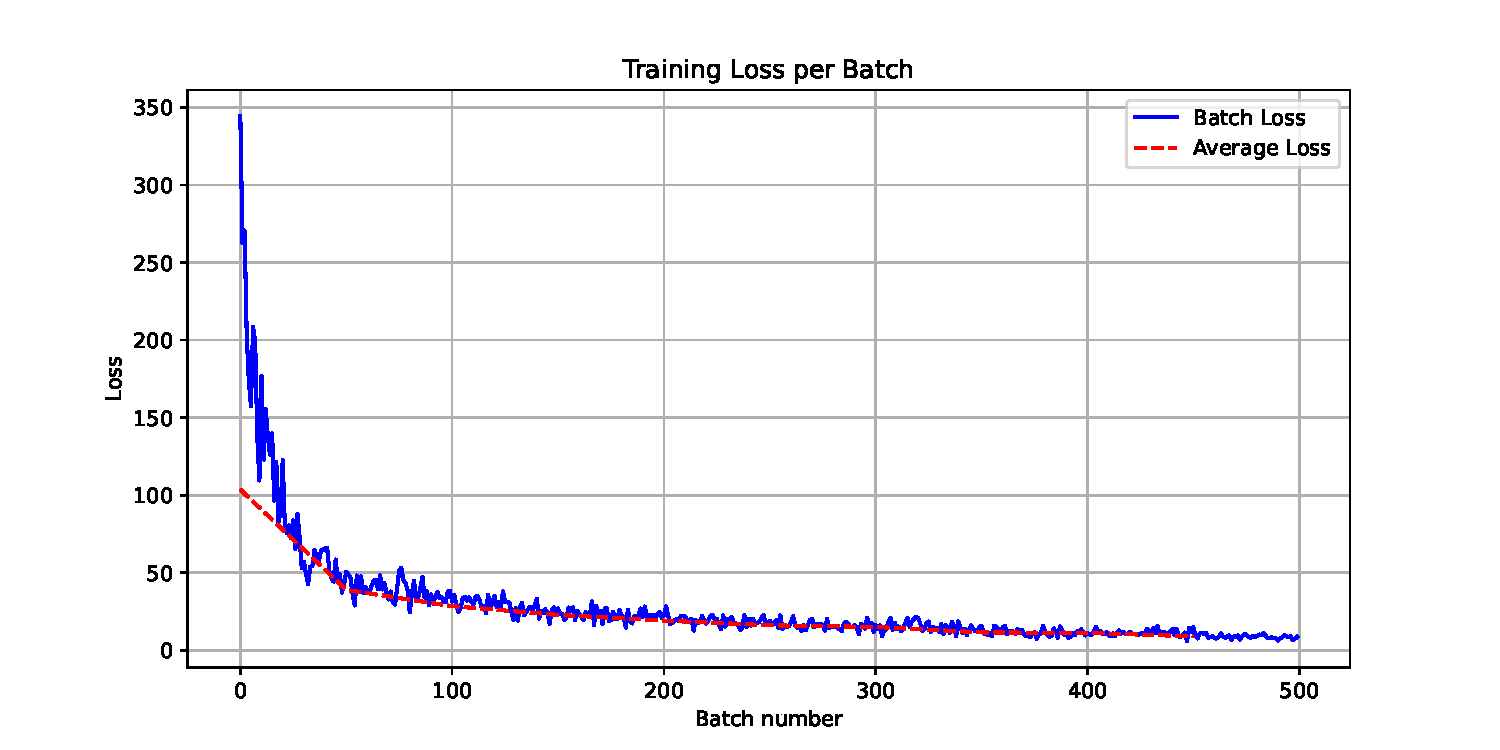
\includegraphics[width=\textwidth]{figures/batch_loss_curve.pdf}
    \caption{Крива тренування нейронної мережі на основі конволюційних шарів 
    Колмогорова-Арнольда (CKAN).}
    \label{fig:train-curve}
\end{figure}
